\section{Evaluation}

In this section we present an evaluation of our approach. Our evaluation comprises two parts: (i) a usability evaluation involving two experiments with two groups of students (Section~\ref{sec:usab}); and (ii) a preliminary analysis of the performance overhead of our approach (Section~\ref{sec:perf}). The exact input, instructions, and any additional document we have used in this section should be available at \cite{repo}.

\subsection{Usability Evaluation}\label{sec:usab}

We ran empirical evaluation to measure the efficiency of deadlock exceptions with regards to problem solving speed and accuracy. We defined two research questions for this evaluation: {\bf RQ1.} Is the time spent to identify the bug reduced using our implementation? {\bf RQ2.} Is the accuracy of bug description improved for implementation with deadlock exception when compared to the default one? To answer the first question, we watched for the time (in seconds) to finish each task. For the second question, each answer was evaluated based on three criteria with three possible values each: 0 for absence, 0.5 for partially present and 1 for fully present. Whenever $(A - B) + C \geq 1.5$ was true, we defined it as a correct answer, that is, whenever the bug was described as deadlock and at least one of the methods involved in the deadlock were identified correctly.

\begin{table}
\begin{center}
\caption{Criteria evaluated for each answer}
\begin{tabular}{|l|l|}
\hline
Type & Description \\
\hline
A & Correctly classified problem as deadlock.\\
B & Classified problem as different from deadlock.\\
C & Correctly identified method calls involved in the deadlock.\\
\hline
\end{tabular}
\end{center}
\end{table}

We wrote two programs with different complexity which were presented in the same order for all subjects. The first program, known as \emph{Bank}, contained 4 classes spread in 4 files, 3 threads, 3 explicit locks, and 82 lines of code in average. The second program, known as \emph{Eclipse} had 15 classes spread in 11 files, 4 threads, 5 explicit locks, and 40 lines of code in average. We expected the first program to be easier to identify the deadlock because it contained fewer classes and files. Each program could use either \emph{LockA} or \emph{LockB}, where \emph{LockA} was our implementation with deadlock detection on at least one thread involved in a deadlock, while \emph{LockB} was just the default \emph{ReentrantLock} implementation. Each student was assigned to either group A or B randomly. In group A, student would start with \emph{LockA} in the first program but use \emph{LockB} on the second program; meanwhile, in group B students would have the locks in opposite order.

All students started the experiment with the first question containing \emph{Program 1}. When they finish to provide an answer, they should request for the second question. In this case, we collect the assignment, set a timestamp on it, and deliver second question with \emph{Program 2}. Timestamp was written based on a chronometer visible to everyone in the laboratory.
We set time limit for each question as 60 min, but the first group requested more time and we expanded to 90 min each. 

We ran this experiment with two groups in two different days. First group consisted of undergraduate students attending Programming Language Paradigms course; they had classes about concurrent programming, including exercises in Java using \emph{ReentrantLock} where deadlocks and other concurrent bugs should be avoided; however, these students were not experienced. Second group had graduate students enrolled in master's degree or PhD program attending Parallel Programming course; they had classes about advanced concepts of parallel programming and had practical exercises, including implementing their own lock; consequently they were expected to be very experienced in detecting concurrency bugs.

\subsubsection{Time Analysis.}

We defined the following hypothesis to answer {\bf RQ1}:

\begin{equation}
  H_{0} : \mu_{TimeLockA} \geq \mu_{TimeLockB}
\end{equation}
\begin{equation}
  H_{1} : \mu_{TimeLockA} < \mu_{TimeLockB}
\end{equation}

We used Latin Square Design to control two factors that might affect the metrics: subjects and program complexity.
We designed one program that we considered easy to identify the bug even without exceptions and another program that was more difficult, composed by many files and classes and reflecting a more realistic case. We provided implementations of each program using either \emph{LockA} or \emph{LockB}: the two possible treatments we wanted to compare. Since we had N subjects, 2 programs and 2 possible treatments, we disposed subjects in rows and programs in columns of latin squares, randomly assigning in each cell of the square a treatment that could be \emph{LockA} or \emph{LockB}, but also guaranteeing that for any given row or column in this square, each treatment appears only once. Consequently, we have replication, local control and randomization which are the three principles of experiment design \cite{box}. Time analysis was conducted with R Statistical Software using the inputs extracted from each day. We used the linear model described in Figure~\ref{fig:model} that considers the effect of different factors on the response variable similarly to Accioly's work\cite{paola}, adding the effect between each replica and treatment \cite{sanchez}.

\begin{figure}
\begin{center}
$Y_{lijk} = \mu + \tau_{l} + \tau\alpha_{li} + \beta_{j} + \gamma_{k} + \tau\gamma_{lk} + \epsilon_{lijk}$\\
\vspace{4mm}
\begin{tabular}{ll}
$Y_{lijk}$ & - response of $l_{th}$ replica, $i_{th}$ student, $j_{th}$ program, $k_{th}$ lock \\
$\tau_{l}$ & - effect of $l_{th}$ replica \\
$\tau\alpha_{li}$ & - effect of interaction between $l_{th}$ replica and $i_{th}$ student \\
$\beta_{j}$ & - effect of $j_{th}$ program \\
$\gamma_{k}$ & - effect of $k_{th}$ lock \\
$\tau\gamma_{lk}$ & - effect of interaction between $l_{th}$ replica and $k_{th}$ lock \\
$\epsilon_{lijk}$ & - random error \\
\end{tabular}
\caption{Regression model.}\label{fig:model}
\end{center}
\end{figure}

Initially, we plotted box-plot graphics shown in Figure~\ref{fig:boxplot} for both experiments. Then we run Box-Cox transformation to reduce anomalies such as non-additivity and non-normality. The value of $\lambda$ at the maximum point in the curve drawn by box-cox function in R was not approximately 1 ($\lambda = 5$), thus we should apply the transformation: on our regression model, $Y_{lijk}$ should be powered to $\lambda$. We did the same on the second experiment as $\lambda = 1.3636$.

\begin{figure}%
    \centering
    \subfloat[First experiment]{{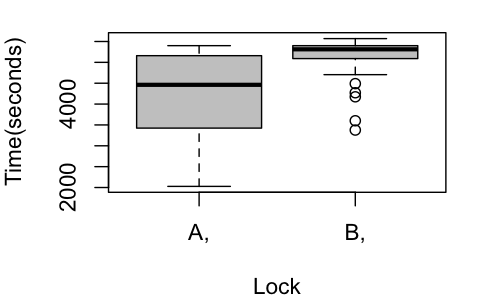
\includegraphics[width=5cm]{img/u1.png} }}%
    \qquad
    \subfloat[Second experiment]{{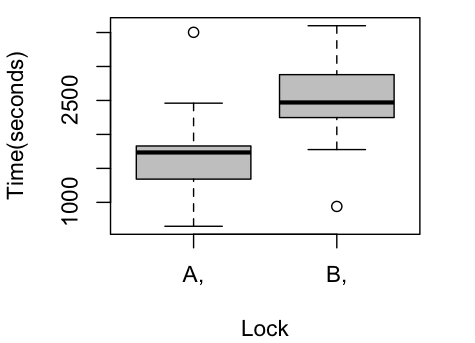
\includegraphics[width=5cm]{img/g1.png} }}%
    \caption{Box-plot on both experiment days}%
    \label{fig:boxplot}%
\end{figure}

After applying Box-Cox transformation, we ran Tukey Test of Additivity that checks whether effect model is additive, so we could evaluate whether interaction between factors displayed on the rows and columns of each latin square wouldn't affect significantly the response when the model is additive \cite{box}. Considering the following hypothesis, in the first experiment, we obtained a p-value of 0.514 which is not lower than 0.05 thus we couldn't reject $H_{0}$, thus our model was additive; similarly for the second experiment, the model was also additive as p-value found was 0.914.

\begin{tabular}{ll}
$H_{0}$ & : The model is additive \\
$H_{1}$ & : $H_{0}$ is $false$ \\
\end{tabular}

Finally, we ran the ANOVA (ANalysis Of VAriance) test which compares the effect of treatments on the response variable, providing an approximated p-value for every associated factor. When a variable has \emph{p-value} $< 0.05$, it means that factor was significant to the response. Table~\ref{tab:unova1} and Table~\ref{tab:unova2} shows the most important factor as the type of \emph{Lock} for both experiments, allowing us to reject our null hypothesis defined for {\bf RQ1}.

\begin{table}%
\begin{center}
\caption{First experiment ANOVA results.}\label{tab:unova1}
\begin{tabular}{|l|l|l|l|l|ll|}
\hline
                & Df &    Sum Sq  &  Mean Sq   & F value & \emph{p-value} &     \\  
Replica         & 14 & 3.8633e+37 & 2.7595e+36 & 1.6553  & 0.1784197 &     \\   
Program         & 1  & 4.1460e+36 & 4.1460e+36 & 2.4869  & 0.1371197 &     \\   
Lock            & 1  & 3.9489e+37 & 3.9489e+37 & 23.6873 & 0.0002492 & *** \\
Replica:Student & 15 & 4.1013e+37 & 2.7342e+36 & 1.6401  & 0.1808595 &     \\  
Replica:Lock    & 14 & 2.4033e+37 & 1.7166e+36 & 1.0297  & 0.4785520 &     \\  
Residuals       & 14 & 2.3340e+37 & 1.6671e+36 &         &           &     \\
\hline
\end{tabular}
\end{center}
\end{table}

\begin{table}%
\begin{center}
\caption{Second experiment ANOVA results.}\label{tab:unova2}
\begin{tabular}{|l|l|l|l|l|ll|}
\hline
                 & Df &    Sum Sq &   Mean Sq  & F value &   Pr(>F) & \\   
\hline
replica          & 6 & 2576883250 &  429480542 & 14.1891 & 0.0025793 & **  \\
program          & 1 &    6875586 &    6875586 &  0.2272 & 0.6505035 &     \\
lock             & 1 & 1958179433 & 1958179433 & 64.6938 & 0.0001975 & *** \\
replica:student  & 7 & 2328154077 &  332593440 & 10.9881 & 0.0047601 & **  \\
replica:lock     & 6 &  823830276 &  137305046 &  4.5362 & 0.0441188 & *   \\
Residuals        & 6 &  181610625 &   30268438 &         &           &     \\
\hline
\end{tabular}
\end{center}
\end{table}

\subsubsection{Accuracy Analysis.}

We used the number of correct answers using each lock to measure accuracy, so we defined the following hypothesis to answer {\bf RQ2}. 

\begin{equation}
  H_{0} : \mu_{CorrectAnswersLockA} \leq \mu_{CorrectAnswersLockB}
\end{equation}
\begin{equation}
  H_{1} : \mu_{CorrectAnswersLockA} > \mu_{CorrectAnswersLockB}
\end{equation}

\begin{table}
\parbox{.45\linewidth}{
\centering
\begin{tabular}{|l|l|l|}
\hline
 & Correct & Incorrect\\
\hline
LockA & 29 & 2\\
LockB & 16 & 15\\
\hline
\end{tabular}
\caption{First group accuracy}\label{tab:accuracy1}
}
\hfill
\parbox{.45\linewidth}{
\centering
\begin{tabular}{|l|l|l|}
\hline
 & Correct & Incorrect\\
\hline
LockA & 13 & 1\\
LockB & 10 & 4\\
\hline
\end{tabular}
\caption{Second group accuracy}\label{tab:accuracy2}
}
\end{table}

Applying Fisher's exact test on data from Table~\ref{tab:accuracy1} and Table~\ref{tab:accuracy2}, we can see that undergraduate students results presented a two-tailed P value equals 0.0004: the association between rows (groups) and columns (outcomes) was considered to be extremely statistically significant; consequently, it's an evidence of improvement on accuracy. However graduate students results presented a two-tailed P value equals 0.3259, which does not represent a statistically significant evidence.

% TODO: add script and the data used (anonymized) to appendices or put on github and link %

\subsubsection{Discussion}

Although we cannot draw conclusions regarding improved accuracy, we found some interesting behavior. Some students in the second group were greatly experienced on concurrent programming and they knew how to efficiently find a deadlock using the tools available in Eclipse, thus being able to finish the tasks really quickly for both problems knowing exactly which points in the code were involved in the deadlock. This observation allows us to hypothetize whether deadlock exceptions are more helpful for less experienced programmers in general, but we leave this as a proposal for future work.

\subsubsection{Threats to Validity}

We must consider a few remarks regarding the validity of our results. First remark is about the way we collected the timestamps: when a student finished any question, we manually wrote their name with the timestamp on the whiteboard so we could track time limit individually later, but we could potentially reduce overhead and increase timestamps precision if we used an automated alternative.
Secondly, the first group did this experiment in replacement of their actual exam might have impacted the time we measured. We noticed some students spent more time on each question by purpose. We believe that they were reluctant to ask for the next question because they still had plenty of time left and they wanted to make sure it was correct. We did not notice such behavior with the second group of students and we believe it is because they did not have the same pressure to deliver correct results as the first group had.
Third remark is related to programs' complexity: the ones we used to evaluate the students are considerably easier to understand than most programs in real world, but unfortunately we could not use any real world scenario as students would not be able to finish each assignment in time; with that in mind, we created two questions based on real world bugs we found on our bug report studies.
Forth remark is about different background over different subjects: we tried to minimize their background differences by selecting groups where students had at least basic experience in concurrent programming and they should be familiarized with the types of bugs such codes could have; the first group was composed by undergraduate students who attended the class \emph{Paradigms of Computaional Languages} where deadlocks were covered in classes and exercises; meanwhile, the second group had graduate students who attended the class \emph{Parallel Programming} which covered concurrent programming in low level detail including deadlock detection. Last remark is about whether we are able to draw conclusions based on students data: some studies suggest that using students as subjects is as good as using industry professionals \cite{staron}; Runes ran an experiment which shows that there's not much significant differences between undergraduate, graduate and industry professionals, with the exception that undergraduate students often take more time to complete the tasks \cite{runes}.

\subsection{Performance Overhead}\label{sec:perf}

We conducted a preliminary set of experiments to analyze the overhead of our approach. We compared our deadlock-safe implementation with the original {\tt ReentrantLock} implementation available in the JDK and with Eclipse's deadlock-safe {\tt OrderedLock} \cite{orderedlock}. {\tt OrderedLock} is similar our approach in the sense that it attempts to detect deadlocks at runtime. However, it aims to be general, detecting $N$-thread deadlocks without much concern for performance. 
OrderedLock deeply relies on Eclipse's code architecture. So, in order to use it in our evaluation, we had to perform some small code changes, removing only Eclipse-specific bits that did not affect the core functionality of {\tt OrderedLock}. The source code for these lock implementations is available elsewhere\cite{repo}.

We developed a synthetic benchmark that creates \emph{N} threads that perform additions to ten integer counters where each increment in a counter is protected by explicit locks. Each thread would have to increment its corresponding counter 1000 times before finishing its execution and the counters were evenly distributed across the threads. Therefore, each counter will have exactly \emph{(N / 10)} threads doing increments on it and higher values of \emph{N} result in higher contention, that is, more threads will compete against each other for a particular counter. In this preliminary evaluation, we have conducted measurements for values of $N$ equal to 10, 50, 100, and 200. Since each thread in the benchmark never acquires more than one lock at the same time, deadlocks cannot occur. We emphasize that this setup is very conservative, since every operation that each thread performs requires locking. Thus, the obtained overhead will be a worst-case estimate and thus much higher than one would encounter in a real-world application~\cite{lozi}. 

The measurements were made on an Intel CoreTM i7 3632QM Processor (6Mb Cache, 2.2GHz) running Ubuntu 12.04.4 LTS and each cell in Table~\ref{tab:overhead} is the average of 50 executions (preceded by 20 executions that served as a warm-up). 

\begin{table}
\begin{center}
\caption{Benchmark time measurements (in seconds)}\label{tab:overhead}
\begin{tabular}{|l|l|l|l|}
\hline
\# Threads & ReentrantLock & ReentrantLock Modified & OrderedLock \\
\hline
10 & 0.084184 & 0.105729 & 0.159503\\
50 & 0.089094 & 0.136507 & 1.094718\\
100 & 0.090978 & 0.159541 & 3.395974\\
200 & 0.131739 & 0.194075 & 11.258714\\
\hline
\end{tabular}
\end{center}
\end{table}

The difference of results between our implementation and the original ReentrantLock gives a range of increased time from about 50\% to 90\%. Meanwhile, OrderedLock performed a lot worse, reaching a 8446.3\% increase in time for the worst case. 

To get a rough estimate of the impact that this overhead would have on actual application execution time, we analyzed the results obtained by Lozi et al.~\cite{lozi}. The authors profiled 19 real-world applications and small benchmarks in order to measure the time these systems spend on their critical sections. Worst-case results ranged between 0.3\% and 92.7\%. If we consider the average time spent on the critical sections of 12 of these systems, the impact of our approach on the overall execution time would be \textbf{less than 6\% in the worst case}. The remaining cases are extreme, in the sense that these systems spend more time in their critical sections than out of them~\cite{lozi}. 

